% IEEE T-ITS submission draft: two-column, single-spaced journal format.
% Compile from paper/ with: latexmk -pdf main.tex
\documentclass[journal]{IEEEtran}

\usepackage{cite}
\usepackage{amsmath,amssymb}
\usepackage{graphicx}
\usepackage{tikz}
\usetikzlibrary{arrows.meta}

\title{Forensic Reconstruction of Road Collisions from Independent Onboard Recordings}

\author{Lorenzo Bacchiani, Andrea Bedei, Mario Bravetti, Roberto Girau, and Giovanni Pau%
\thanks{L. Bacchiani, A. Bedei, M. Bravetti, R. Girau, and G. Pau are with the University of Bologna, Bologna, Italy.}}

\begin{document}

\maketitle

\begin{abstract}
Road collisions are often observed only through partial recordings made by the vehicles involved. This paper presents a retrospective method that aligns multiple onboard recordings, associates radar tracks across observers, reconstructs road users without their own recordings, and derives a shared semantic event trace. The evaluation examines reconstruction quality and robustness to positioning and radar errors in simulated collision scenarios.
\end{abstract}

\begin{IEEEkeywords}
Partial observability, collision reconstruction, automotive radar, multi-vehicle fusion, forensic analysis.
\end{IEEEkeywords}

\section{Introduction}
\label{sec:introduction}

% Motivate retrospective reconstruction from partial onboard recordings.
% State the problem, the information available to each recorder, and the
% contributions. Keep responsibility judgments with the human investigator.

\section{Running Example}
\label{sec:running-example}

% Use one canonical collision to introduce recorder-local observations,
% a road user without a recorder, the reconstructed scene, and event timing.
% Draw the example from one frozen code version and its matching results.

\section{Background}
\label{sec:background}

\subsection{State Estimation: Filtering and Smoothing}
\label{subsec:state-estimation}

State estimation infers the motion of an object from noisy observations.
For planar vehicle motion, a common state contains position and velocity,
$\mathbf{x}_k=(p_x,p_y,v_x,v_y)^{\mathsf T}$, at sampling instant $k$.
For Cartesian position and directional velocity measurements, a linear
state-space model describes its evolution and observation as
\begin{equation}
  \mathbf{x}_k=\mathbf{F}_k\mathbf{x}_{k-1}+\mathbf{w}_k,
  \qquad
  \mathbf{z}_k=\mathbf{H}_k\mathbf{x}_k+\mathbf{v}_k,
  \label{eq:state-space}
\end{equation}
where $\mathbf{F}_k$ models motion, $\mathbf{H}_k$ relates the state to the
measurements, and $\mathbf{w}_k$ and $\mathbf{v}_k$ represent process and
measurement noise, with covariances $\mathbf{Q}_k$ and $\mathbf{R}_k$.
In a constant-velocity model, position advances by velocity times the
sampling interval; process noise accounts for departures from that
prediction, including acceleration~\cite{barshalom2001estimation}.

The Kalman filter recursively propagates a state estimate and its error
covariance, then updates them using the next measurement and its
uncertainty~\cite{kalman1960filtering}. Filtering estimates the state at
$k$ using observations through $k$. Fixed-interval smoothing estimates
that same state using the entire observation sequence, including later
measurements. The Rauch--Tung--Striebel (RTS) smoother performs a backward
recursion over the filtered estimates~\cite{rauch1965smoothing}.
This distinction is relevant to retrospective analysis, where the complete
recording is available. Both estimates depend on the assumed motion model;
an abrupt velocity change at impact requires that assumption to be revisited.

\subsection{Multi-Object Tracking and Data Association}
\label{subsec:multi-object-tracking}

Multi-object tracking estimates several trajectories while maintaining
their identities over time. Sensor detections generally carry no reliable
object identity: a vehicle can produce several returns, disappear from
view, or pass close to another vehicle. Data association determines which
observations belong to which tracks, while track management handles their
initiation, continuation, and termination~\cite{barshalom2001estimation}.
For a predicted state $\hat{\mathbf{x}}$ with covariance $\mathbf{P}$,
the measurement innovation $\mathbf{r}=\mathbf{z}-\mathbf{H}\hat{\mathbf{x}}$
has covariance $\mathbf{S}=\mathbf{H}\mathbf{P}\mathbf{H}^{\mathsf T}+\mathbf{R}$.
Compatibility can be assessed using the squared Mahalanobis distance,
\begin{equation}
  d^2=\mathbf{r}^{\mathsf T}\mathbf{S}^{-1}\mathbf{r}.
  \label{eq:association-distance}
\end{equation}
A statistical gate rejects incompatible candidates. Passing the gate
establishes compatibility, but several tracks may still explain the same
observation.

Automotive radar also requires an extended-object view of a vehicle.
Multiple detections can arise from spatially separated reflection centres,
and their distribution depends on the visible parts of the
body~\cite{hammarstrand2012extended}. Doppler measures relative velocity along each
return's line of sight; a single return does not directly determine the
tangential component. Consequently, a tracked radar position need not
coincide with the vehicle centre, and different observers can track
different surfaces of the same car. Extended-object tracking explicitly
accounts for the relationship between object motion, physical extent,
and multiple detections~\cite{granstrom2017extended}.

With several observers, association also operates between tracks.
A local track label identifies an observation history within one source;
track-to-track association determines whether histories from different
sources describe the same physical object. Establishing that correspondence
and fusing the associated state estimates are distinct estimation
problems~\cite{chong2000association}.

\subsection{Traffic Conflict Measures}
\label{subsec:traffic-conflicts}

Traffic-conflict measures quantify proximity to a collision under specified
motion assumptions. Time to collision (TTC) is the time until the first
predicted contact if those assumptions continue to
hold~\cite{hayward1972near-miss}. For two vehicles following a straight path
at constant speeds, with follower speed $v_f>v_l$ and leader speed $v_l$,
TTC and the following time gap are
\begin{equation}
  \mathrm{TTC}=\frac{d}{v_f-v_l},
  \qquad
  \tau_{\mathrm{gap}}=\frac{d}{v_f},
  \label{eq:ttc-time-gap}
\end{equation}
where $d>0$ is the bumper-to-bumper clearance. The latter is a net time gap;
gross time headway instead uses front-to-front spacing. These measures
describe different properties: two vehicles travelling at the same speed
can have a short following gap while their constant-speed TTC is infinite.
Close following and an imminent collision are therefore distinct
conditions~\cite{vogel2003headway}.

For cut-ins and crossing traffic, the distance-to-closing-speed ratio alone
does not establish a collision course. Predictions must account for both
vehicles' paths and physical footprints. Measures based on braking further
consider the deceleration needed to avoid predicted contact after an
assumed response delay. Their interpretation depends on the motion model,
response assumptions, and available deceleration~\cite{westhofen2023criticality}.
They characterize aspects of conflict urgency without establishing its cause.

Response timing also depends on context. Naturalistic studies show that
braking onset varies with the evolving kinematic urgency of an encounter,
rather than following a universal delay after a single hazard
onset~\cite{markkula2016braking}. An interval from a conflict observable
in sensor data to brake application describes an observed braking delay;
it does not establish when the driver perceived the hazard or whether the
driver was distracted.

\section{Methodology}
\label{sec:methodology}

% Describe local radar tracking and smoothing, clock alignment, recorder
% association, anonymous-road-user fusion, collision matching, and semantic
% event extraction. Specify which inputs each stage may read.

\section{Evaluation}
\label{sec:evaluation}

% Report the frozen scenario set, sensor-error profiles, evaluation oracles,
% absolute and relative pose errors, incident-relevant outcomes, and the
% GNSS-by-radar campaign. Include one commit hash for all final results.
% State the operational positioning bound with its percentile definition.

\section{Related Work}
\label{sec:related-work}

% Compare accident reconstruction, event-data recording, cooperative
% perception, radar tracking, and multi-vehicle localization. Focus on the
% difference between retrospective fusion and live cooperative perception.

\section{Threats to Validity}
\label{sec:threat}
\section{Conclusion}
\label{sec:conclusion}

% Summarize the demonstrated reconstruction capability and its measured
% operating conditions. Keep deployment and responsibility claims within
% the evidence provided by the simulated evaluation.


\bibliographystyle{IEEEtran}
\bibliography{references}

\begin{IEEEbiography}[{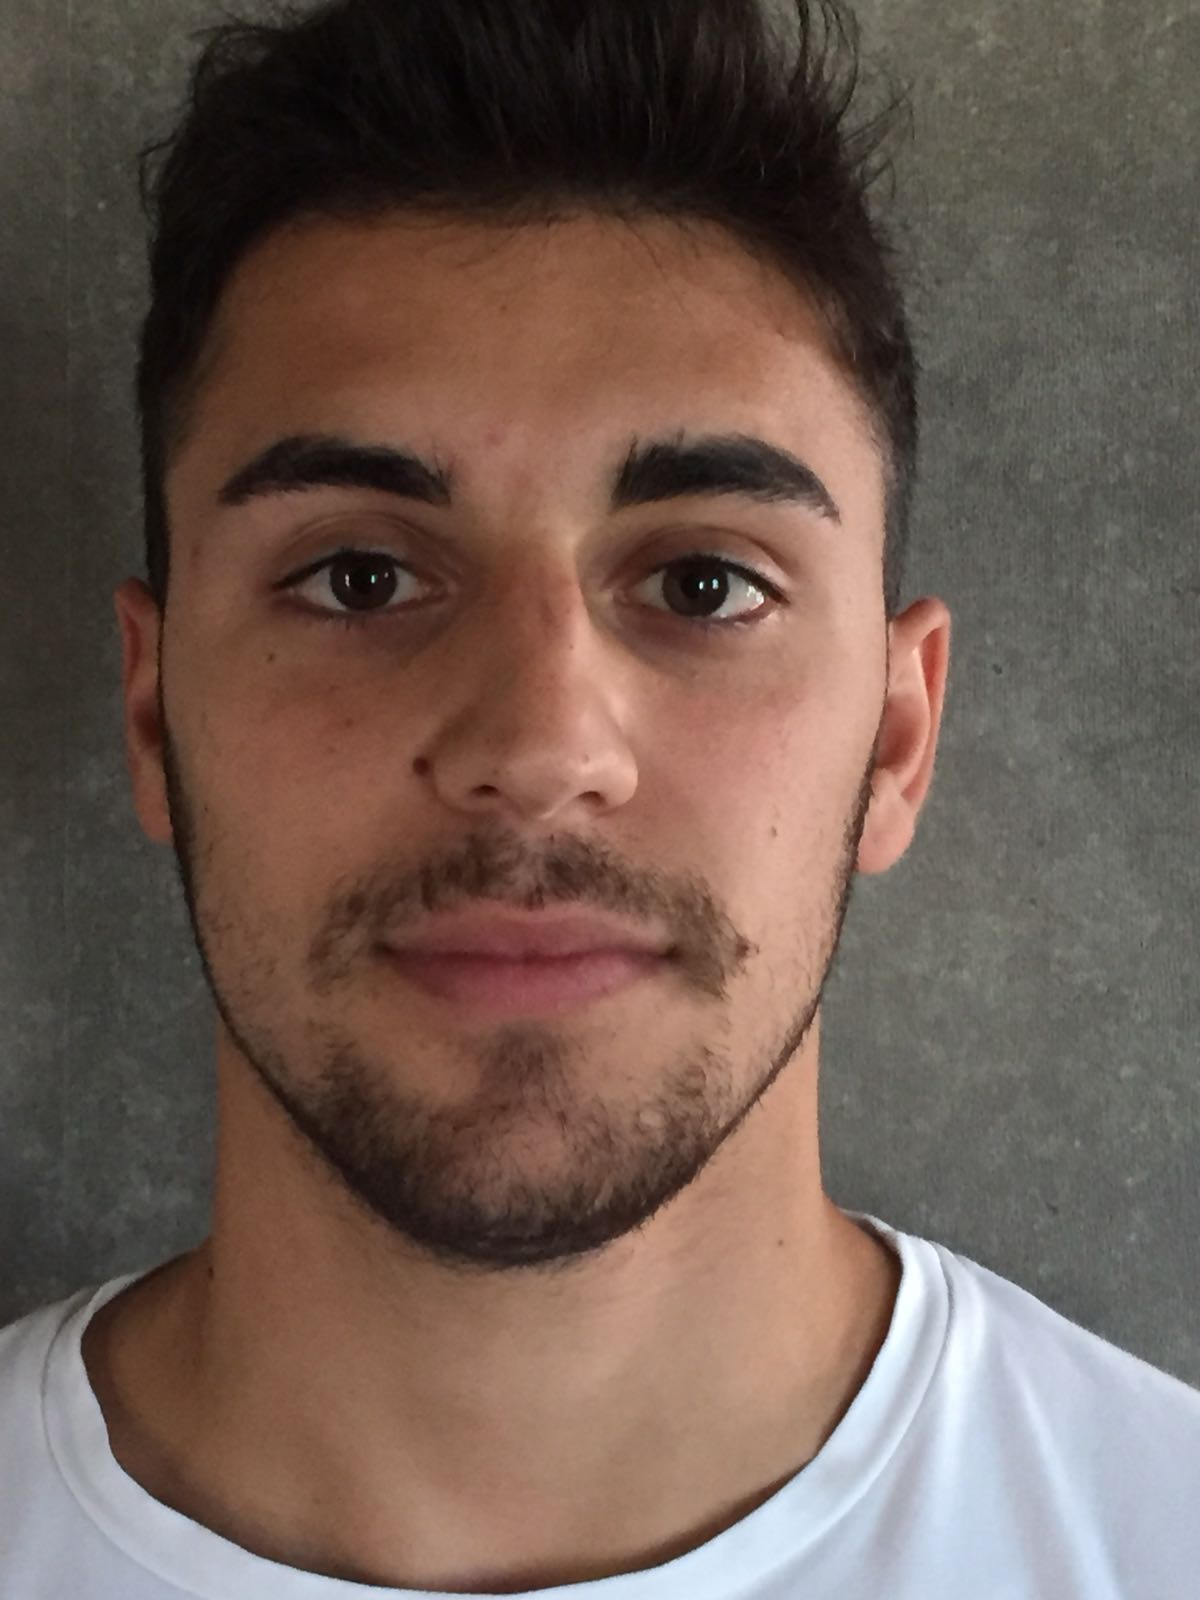
\includegraphics[width=1in,height=1.25in,clip,keepaspectratio]{figures/bacchiani.jpeg}}]{Lorenzo Bacchiani} 
    Lorenzo Bacchiani received his Ph.D. in Computer Science and Engineering from the University of Bologna in 2025. He is currently a 
    Research Fellow at the Department of Computer Science and Engineering, University of Bologna. His  interests include behavioral-based 
    methodologies for component interaction, adaptation, and deployment, as well as digital twin technologies in the automotive domain. 
    In particular, his work explores the development and integration of vehicle, driver and road digital twins to improve system reliability and safety.
\end{IEEEbiography}

\begin{IEEEbiography}[{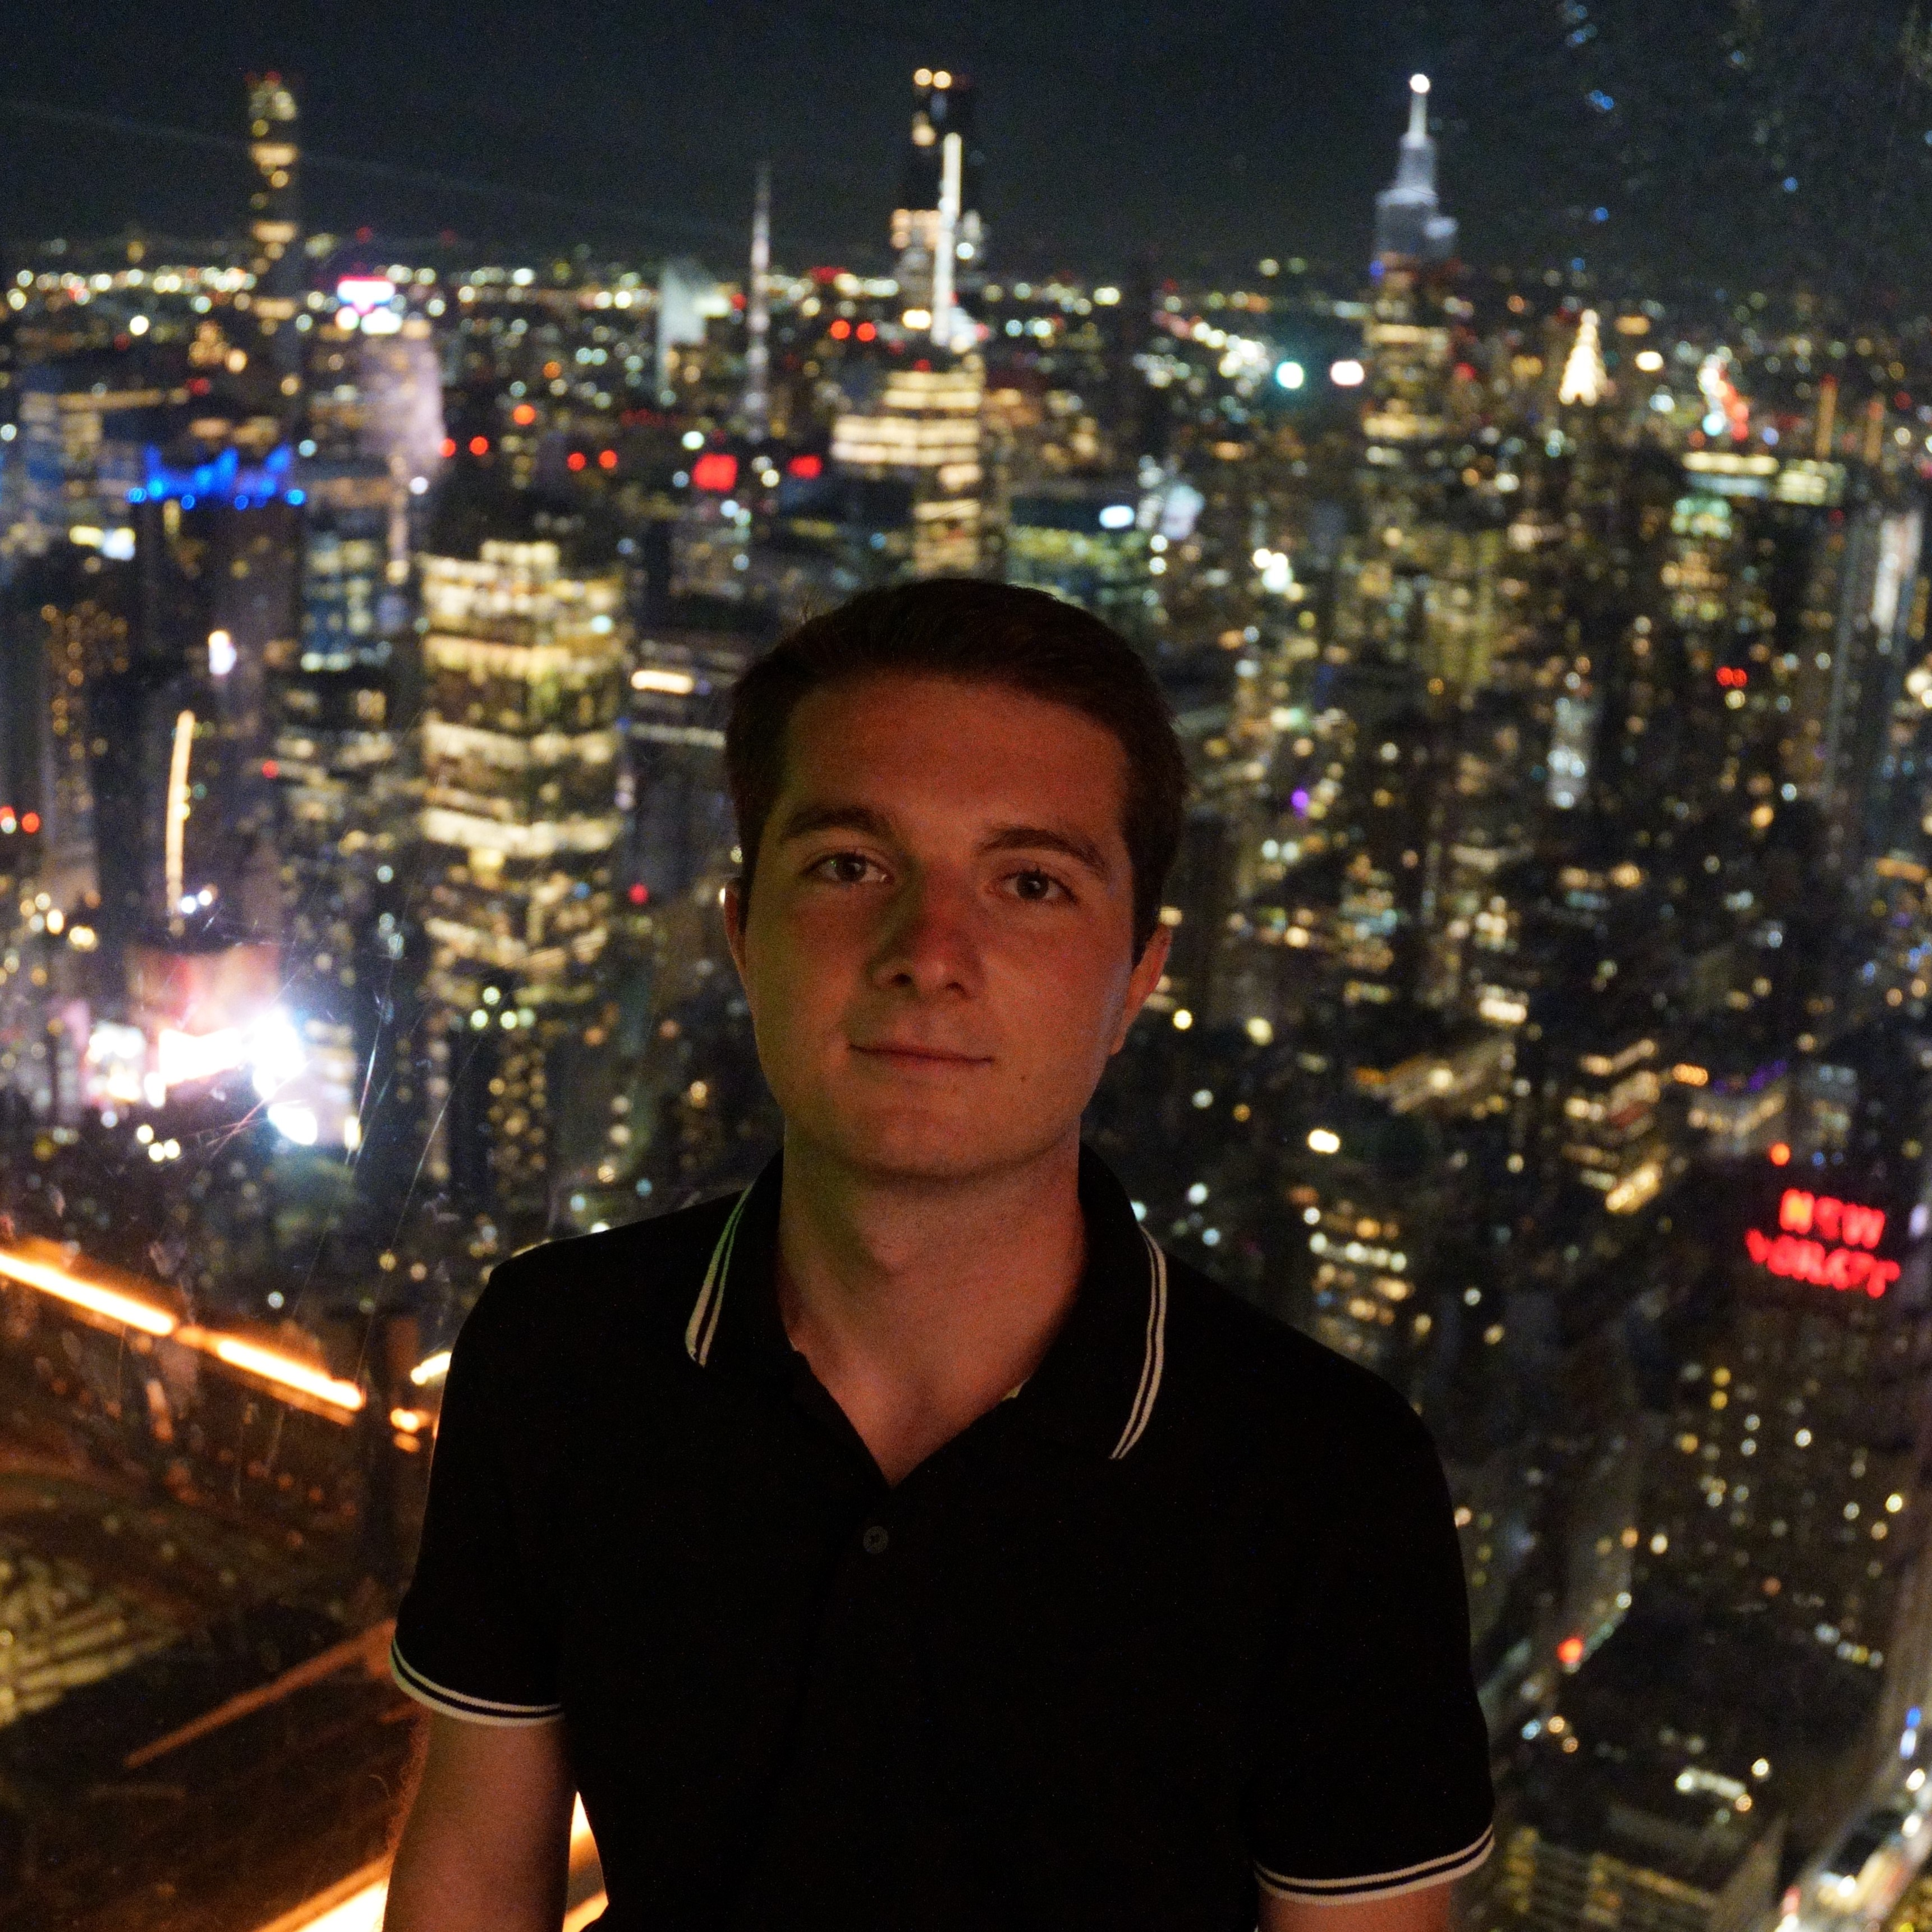
\includegraphics[width=1in,height=1.25in,clip,keepaspectratio]{figures/bedei.JPG}}]{Andrea Bedei}
Andrea Bedei is a Ph.D. candidate in Automotive Engineering for Intelligent Mobility at the University of Bologna, Cesena Campus. He received 
the M.S. degree in Computer Science and Engineering from the same University in 2025. His research interests include computer vision, machine 
learning, simulation frameworks for autonomous vehicle safety, and the use of virtual environments for marine robotics and underwater drone experimentation.
\end{IEEEbiography}


\begin{IEEEbiography}[{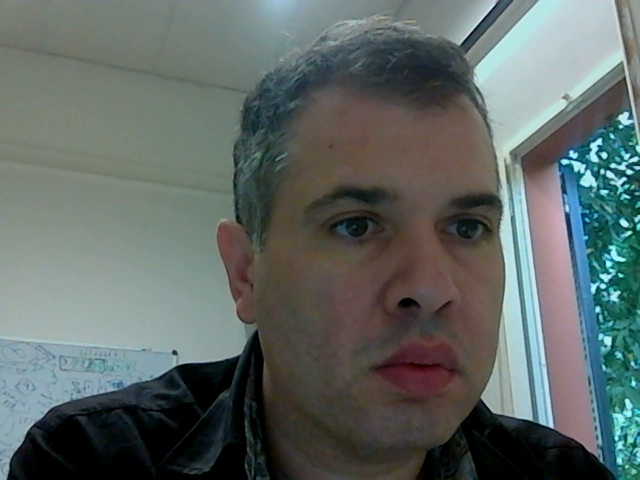
\includegraphics[width=1in,height=1.25in,clip,keepaspectratio]{figures/bravetti.jpeg}}]{Mario Bravetti} Mario Bravetti is a 
    Full Professor at the Department of Computer Science and Engineering of the University of Bologna. His research spans 
    formal methods for distributed systems, concurrency and probability theory, and applications to service-oriented and cloud 
    computing. He has contributed to numerous international research projects, served on editorial boards of international 
    computer science journals, and authored more than 100 peer-reviewed publications. He has held key roles in major international 
    conferences, including CONCUR, SEFM, SAC, and QEST, as well as in several international PhD schools and scientific committees.
\end{IEEEbiography}


\begin{IEEEbiography}[{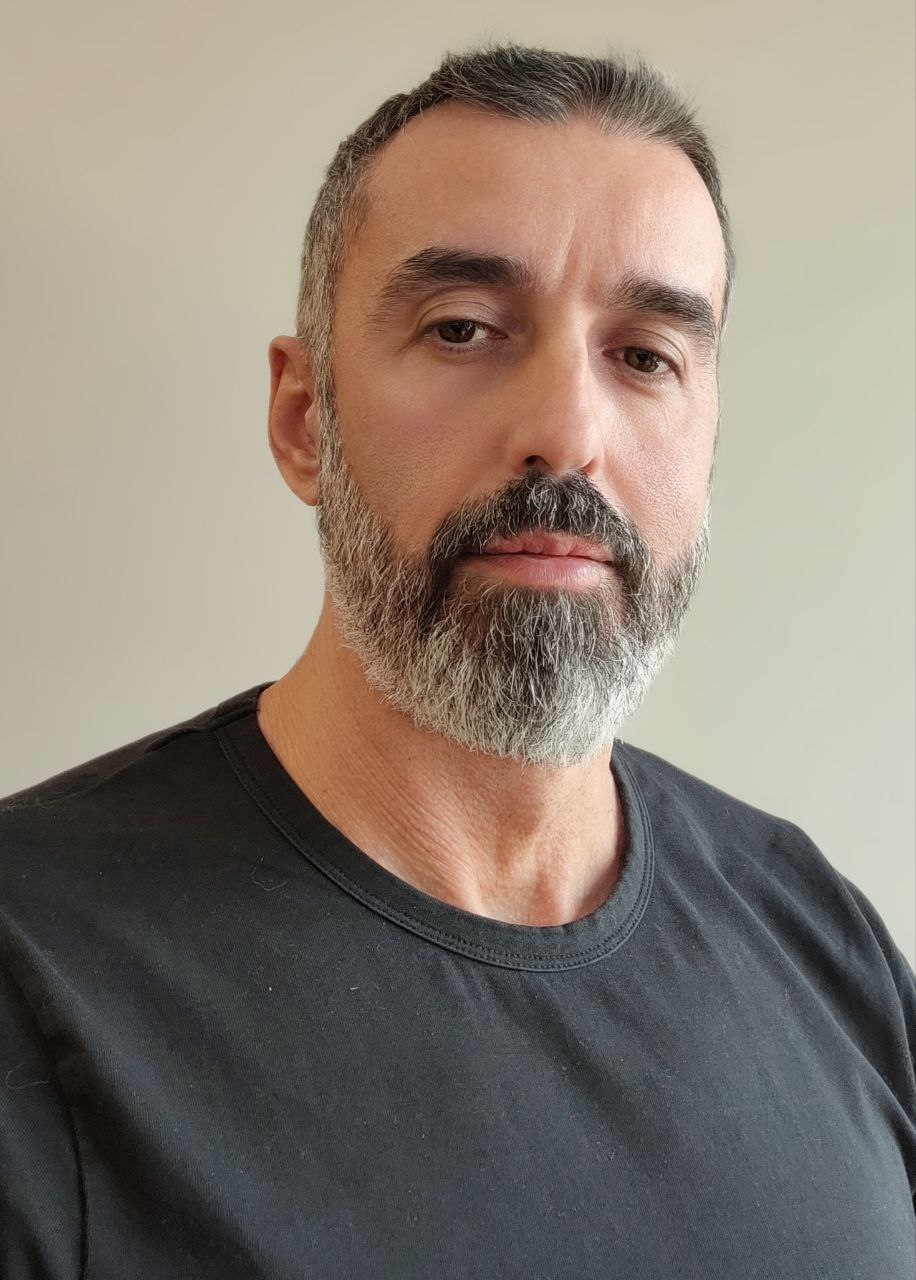
\includegraphics[width=1in,height=1.25in,clip,keepaspectratio]{figures/girau.jpg}}]{Roberto Girau} Roberto Girau (Senior Member, IEEE) 
    is associate professor at University of Bologna, Department of Computer Science and Engineering since 2021. He received the M.S. degree in 
    Telecommunication Engineering and his Ph.D. degree in electronic engineering and computer science from the University of Cagliari, 
    Italy in 2012 and in 2017, respectively. From 2012 to 2020, he worked as researcher at the Department of Electrical and Electronic 
    Engineering of the University of Cagliari, developing an experimental platform for the social Internet of Things. 
    His main research areas of interest are IoT and vehicular and human digital twins with particular emphasis on safety applications.
\end{IEEEbiography}

\begin{IEEEbiography}[{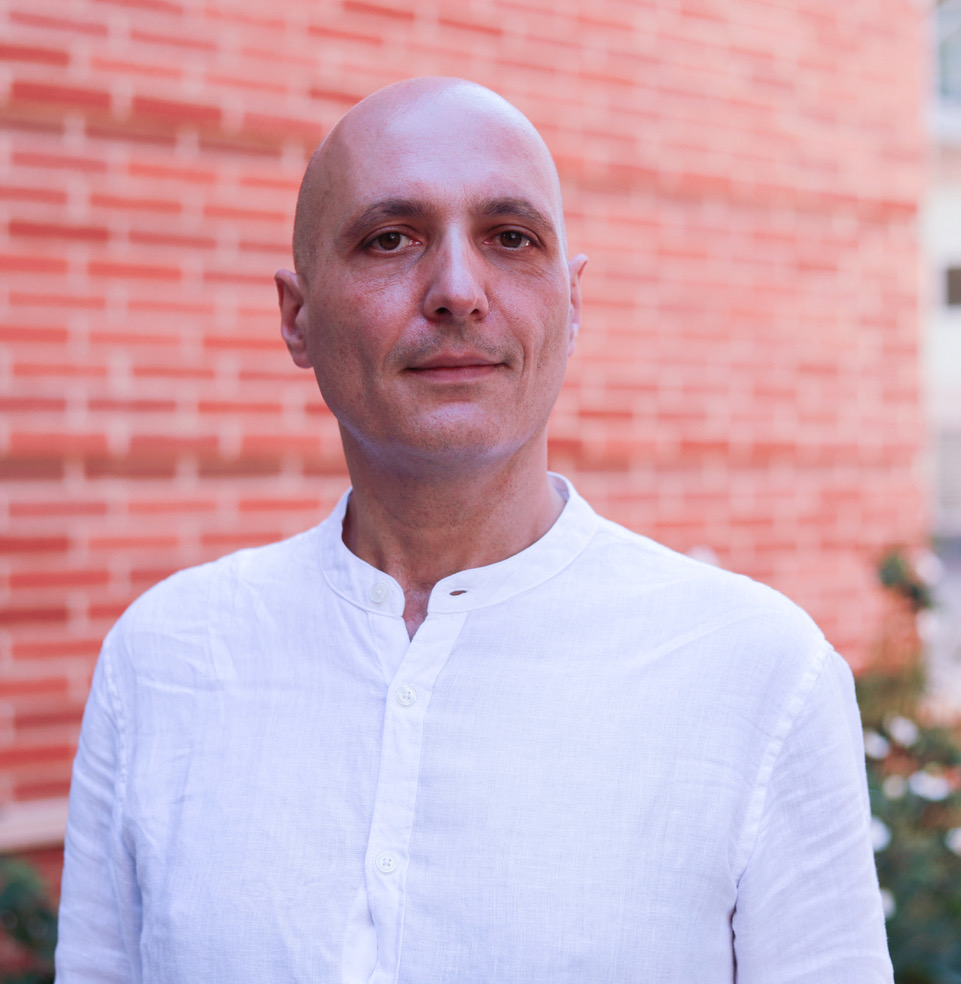
\includegraphics[width=1in,height=1.25in,clip,keepaspectratio]{figures/GPAU-OfficialSmall.jpeg}}]{Giovanni Pau} Giovanni Pau is a full professor at the University of Bologna -  Department of Computer Science and Engineering (DISI). He also serves as Technical Director at the Technology Innovation Institute of Abu Dhabi and  Adjunct Faculty at the University of California, Los Angeles. Previously Dr. Pau served as ATOS/Renault smart mobility chair of excellence Professor at the Sorbonne Université, Paris France.
Dr. Pau received his Laurea in Computer Science and his PhD in Computer Engineering from the University of Bologna in 1998 and 2002 respectively. He completed his “Habilitation à diriger des recherches” (HDR) at Sorbonne Université in 2018.
His research interests focus on vehicular robotics,  IoT, in the past he worked on network systems, particularly vehicular ad-hoc networks (VANETs), pervasive mobile sensor systems, and the application of information-centric networking (ICN) architectures to mobility and vehicular communication.  His work on vehicular networks and mobile edge has been widely cited by the community and reported on in the general media including BBC Radio, Discovery Channel, The Guardian, Wired, Corriere della Sera, and the Italian National Television.
Over the years, he has published more than 100 peer-reviewed journal and conference articles.
\end{IEEEbiography}

\end{document}
